\documentclass[logo,reportComp]{thesis}
\usepackage[cpp,pseudo]{mypackage}
\lstset{language=python}

\title{分布式系统作业三}
\subtitle{远程过程调用}
\school{数据科学与计算机学院}
\author{陈鸿峥}
\classname{17大数据与人工智能}
\stunum{17341015}
\headercontext{分布式系统作业}

\begin{document}

\maketitle

\begin{question}
远程过程调用(RPC)用将网络编程变得非常简单。
根据所学的RPC相关原理,实现客户端-服务器通信,并进行简单的计算如数据库查询、算术计算、数据挖掘、深度学习推导等。
\begin{figure}[H]
\centering
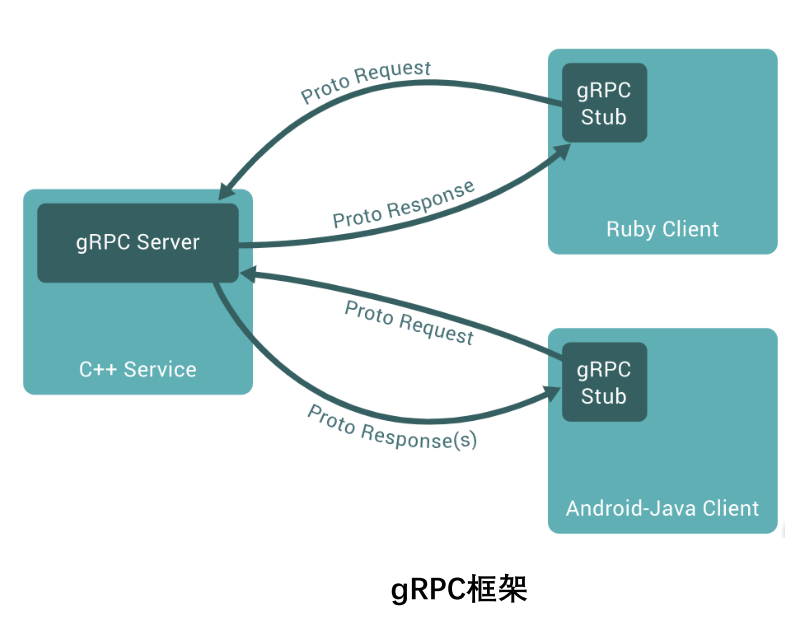
\includegraphics[width=0.6\linewidth]{fig/gRPC-framework.png}
\end{figure}
\begin{itemize}
\item 要求:
\begin{enumerate}
\item 采用gRPC
\item 采用Protobuf作为C-S数据传输格式
\item 服务器端采用线程池,支持并发
\item 支持至少两种的计算服务如简单的算术运算+数据挖掘算法(K-means、KNN等)
\item 编程语言不做要求
\end{enumerate}
\item 建议:gRPC和Protobuf在配置环境时可能有些复杂,对于有些编程语言如C++、Go等会有一些挑战,Python问题会少一些。
\item 关于gRPC的相关例子:\url{https://github.com/grpc/grpc/tree/master/examples}
\end{itemize}
\end{question}

\section{实验内容}
在本次实验中我使用gRPC主要实现了两个功能:\textbf{Python解释器、MySQL查询器}。
客户端设计得与真实的解释器类似,功能也与真实的解释器相似,使得用户即使在本机上没有安装部分Python环境(如numpy/Tensorflow等)或者没有安装MySQL数据库也能够通过远程客户端实现计算、查询等功能。

Python解释器主要采用Python的\textbf{反射}机制(reflection),即\verb'eval'和\verb'exec'。
在客户端方面将用户需要运行的字符串通过gRPC传递给服务器端,服务器端直接对字符串进行运算,并以字符串形式返回给客户端。

而MySQL同样采用类似的机制,客户端通过gRPC将用户输入以字符流的形式传输,服务器端收到后调用\verb'mysql.connector'与数据库建立起链接,并通过MySQL提供的API \verb'execute'语句进行查询,最后将结果返回客户端。

Protobuf文件定义如下(\verb'pyinterpreter.proto'),这里提供两个服务\verb'Evaluation'和\verb'Query',并且共用了字符流格式\verb'EvalRequest'和\verb'EvalReply'。
\begin{lstlisting}[language=c++]
syntax = "proto3";

package pyinterpreter;

service Evaluation {
	rpc eval (EvalRequest) returns (EvalReply) {}
}

service Query {
	rpc query (EvalRequest) returns (EvalReply) {}
}

message EvalRequest {
	string msg = 1;
}

message EvalReply {
	string msg = 1;
}
\end{lstlisting}
定义好后需要使用下列指令对其进行编译,生成对应了类文件,供服务器端和客户端进行调用。
\begin{lstlisting}
python -m grpc_tools.protoc -I. --python_out=. --grpc_python_out=. pyinterpreter.proto
\end{lstlisting}

服务器端(\verb'server.py')主要有以下几个注意点:
\begin{itemize}
	\item \verb'Evaluation'为Python的解释器部分,采用了异常处理方式进行编写。
	先尝试对用户输入的语句进行直接估值(\verb'eval'),并将结果返回。
	如果不行则尝试直接执行(\verb'exec'),这里包括赋值等操作,是没有返回结果的。
	但这里有一个变量作用域和反射的问题。首先由于\verb'Evaluation'只是一个类,其中的函数作用域是局部的,因此调用\verb'exec'生成的用户变量也是局部的,用户很可能没法再次访问;另一方面,直接采用反射的方法进行操作其实是非常危险的,对于一些安全性要求比较高的应用不应该这么做。这两个是目前我的程序中存在的缺陷,但不会影响正常使用。
	\item \verb'SQLQuery'为MySQL的解释器部分。首先需要在服务器端建立起与MySQL数据库的连接,这里采用了yaml进行数据库登录信息的存储,可以有效避免敏感信息泄露,并且具有高度的灵活性。建立连接后对其\verb'cursor'进行\verb'execute'操作,就与普通的数据库查询相似了。
	\item 这里采用了Python的线程池\verb'ThreadPoolExecutor'实现并发操作,在后面的实验中可以看到一个服务器端可以同时连接多个客户端,各个服务互不干扰正常工作。
\end{itemize}
\begin{lstlisting}
from concurrent import futures
import logging
import yaml

import grpc

import numpy as np
import mysql.connector
import pyinterpreter_pb2
import pyinterpreter_pb2_grpc

class Evaluation(pyinterpreter_pb2_grpc.EvaluationServicer):

	def __init__(self):
		print("Created Python interpreter!")

	def eval(self,request,context):
		try:
			msg = str(eval(request.msg))
		except:
			exec(request.msg)
			msg = ""
		return pyinterpreter_pb2.EvalReply(msg=msg)

class SQLQuery(pyinterpreter_pb2_grpc.QueryServicer):

	def __init__(self):
		config = yaml.load(open('config.yaml'))
		print("Connected MySQL '{}'@'{}'!".format(config["user"],config["host"]))
		self.db = mysql.connector.connect(
					  host=config["host"],
					  user=config["user"],
					  passwd=config["passwd"]
					)
		self.cursor = self.db.cursor()

	def query(self,request,context):
		self.cursor.execute("use school;")
		self.cursor.execute(request.msg)
		return pyinterpreter_pb2.EvalReply(msg=str(self.cursor.fetchall()))

def serve():
	server = grpc.server(futures.ThreadPoolExecutor(max_workers=10))
	pyinterpreter_pb2_grpc.add_EvaluationServicer_to_server(Evaluation(),server)
	pyinterpreter_pb2_grpc.add_QueryServicer_to_server(SQLQuery(),server)
	server.add_insecure_port('[::]:50051')
	server.start()
	server.wait_for_termination()

if __name__ == '__main__':
	logging.basicConfig()
	serve()
\end{lstlisting}

Python解释器客户端(\verb'client.py')如下,通过调用生成的gRPC类文件,可以实现传输的功能。同时通过简单的循环输入输出操作,伪造出了一个解释器界面。
\begin{lstlisting}
import logging

import grpc

import pyinterpreter_pb2
import pyinterpreter_pb2_grpc

def run():
	with grpc.insecure_channel('localhost:50051') as channel:
		stub = pyinterpreter_pb2_grpc.EvaluationStub(channel)
		print("gRPC-based Python interpreter")
		while True:
			print(">>> ",end="")
			message = input()
			response = stub.eval(pyinterpreter_pb2.EvalRequest(msg=message))
			if response.msg != "":
				print(response.msg)

if __name__ == '__main__':
	logging.basicConfig()
	run()
\end{lstlisting}

MySQL远程客户端(\verb'clientdb.py')与上述类似。
\begin{lstlisting}
import logging

import grpc

from decimal import Decimal
import pyinterpreter_pb2
import pyinterpreter_pb2_grpc

def run():
	with grpc.insecure_channel('localhost:50051') as channel:
		stub = pyinterpreter_pb2_grpc.QueryStub(channel)
		print("gRPC-based MySQL interpreter")
		while True:
			print("mysql> ",end="")
			message = input()
			response = stub.query(pyinterpreter_pb2.EvalRequest(msg=message))
			if response.msg != "":
				result = eval(response.msg)
				for item in result:
					print(item)

if __name__ == '__main__':
	logging.basicConfig()
	run()
\end{lstlisting}

\section{实验结果}
\begin{figure}[H]
\centering
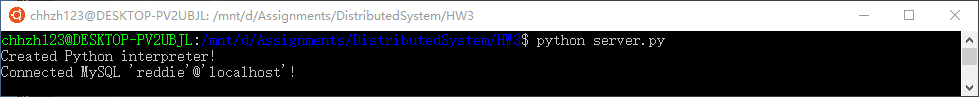
\includegraphics[width=\linewidth]{fig/server.png}
\caption{服务器端,新建服务时会产生提示}
\end{figure}
\begin{figure}[H]
\centering
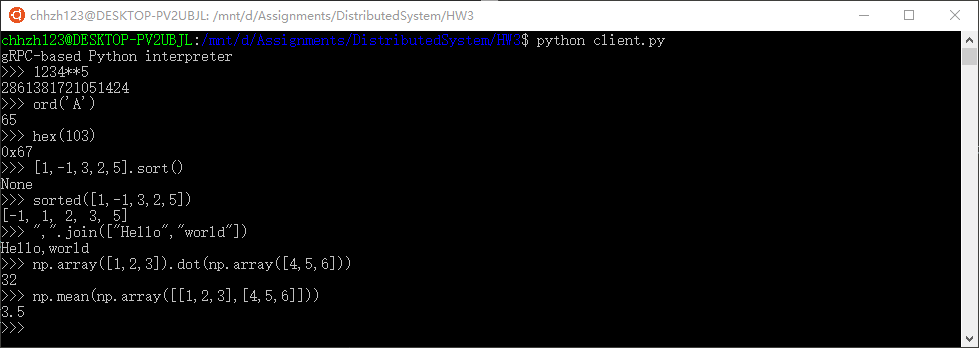
\includegraphics[width=\linewidth]{fig/client.png}
\caption{伪Python解释器客户端,可以实现常见的计算查询服务,并可调用numpy包进行矩阵运算}
\end{figure}
\begin{figure}[H]
\centering
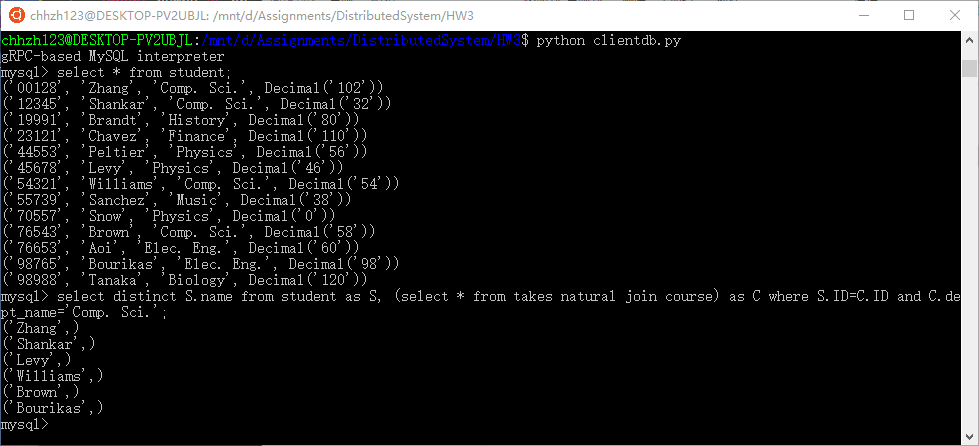
\includegraphics[width=\linewidth]{fig/clientdb.png}
\caption{伪MySQL客户端,可以正常实现复杂数据查询功能,并将查询记录逐行进行显示(这里采用了本学期数据库的school scheme,可用附件中database的文件夹中的sql程序进行生成)}
\end{figure}

遇到的问题及解决方法都已经在前文阐述。
注意要运行我的程序,需要先配置好Python的MySQL连接器,并且按照如下格式配置好yaml文件,才可正常运行。
\begin{lstlisting}[language=c++]
host: // your MySQL host name
user: // your MySQL user name
passwd: // password to login MySQL
\end{lstlisting}

% \begin{thebibliography}{99}
% \end{thebibliography}

\end{document}